\chapter{Introdução}\label{Introducao}
A diversidade de mecanismos químicos catalisados pela enzima terpeno-sintases (TerpS) produz uma variedade larga de terpenos, o produto natural mais antigo e numeroso das plantas. Terpenos são os principais constituintes dos óleos naturais de muitas espécies de plantas. Da mesma forma, por serem compostos voláteis, eles executam um papel crucial em reposta a herbívoros, interação com outras plantas e atração de polinizadores. A quimiodiversidade dos terpenos é esperada como uma característica da vida, levando em conta a biodiversidade considerável de plantas e suas interações com outros organismos. A variedade de terpenos pode ser relacionada à sua função biológica, ajustando-se a quantidade e diversidade destes mesmos terpenos à especificidade do alvo, tanto nas relações de comunicação quanto na proteção contra numerosos predadores, parasitas e competidores. Os benefícios das propriedades dos terpenos para os humanos estendem-se através da utilização deles como temperos em produtos industriais e da agricultura, ou como fragrâncias nas comidas e cosméticos, além dos farmacêuticos e biocombustíveis. Terpenos são nomeados de acordo com o número de unidades de isoprenóides de $C_5$ incorporados em suas cadeias carbônicas como mono- ($C_{10}$), sesqui- ($C_{15}$), di- ($C_{20}$), sester- ($C_{25}$), tri- ($C_{30}$) and sesquarterpenos ($C_{35}$). As unidades de isoprenóides podem ser isopentenilo difosfafto ($IPP$) ou seus isômero alicíclico Difosfato de dimetilalilo ($DMADP$) que são condensados pelas preniltransferases para produzir grande escala de prenil difosfatos, assim como o percursor do monoterpeno geranil difosfato o qual é o mínimo terpeno do substrato de ciclização da biossíntese. Frequentemente, após a perda de geranil difosfato e uma formação de ligação  $C_1-C_6$, a formação de monoterpeno continua ao longo do $\alpha$-terpinil cation por meio de uma cascata de reações as quais incluem ligações $C-C$, rearranjos Wagner-Meerwein,  allyl- and methyl-shifts originados pelas mudanças conformacionais de cátions intermediários, e captura de carbocátion pela água e pelo hidreto.  

\begin{figure}[H]
	\centering
	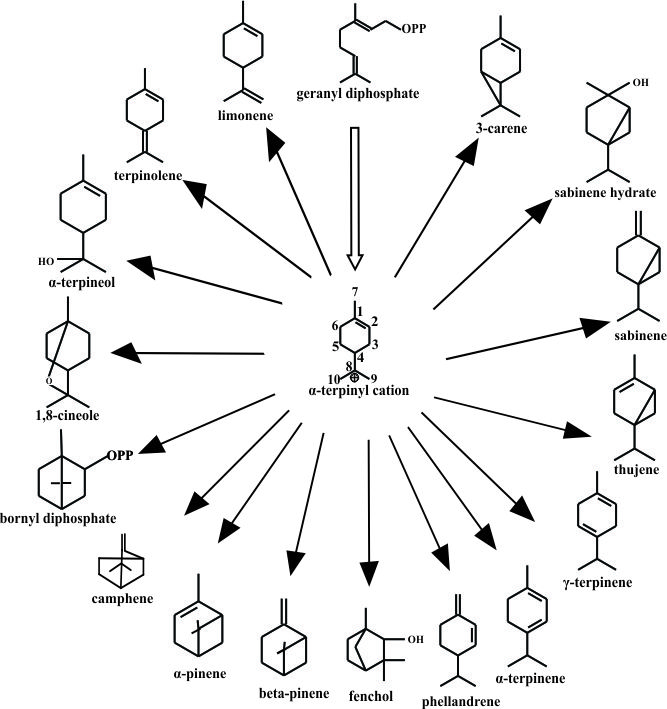
\includegraphics[width=.86\linewidth]{images/img.jpg}
	\caption{{ Exemplos do repertórios de monoterpenos produzidos pelas plantas por meio das ciclizações de Geranil Difosfato ($GPP$)}}
	\label{figIntroCarbocation}
\end{figure}

Há duas diferentes diferentes classes de  (TerpS): Classe I e Classe II definidas cataliticamente por aminoácidos essenciais. As (TerpS) I convertem formas do tipo linear, all-trans, isoprenóides, geranil (C10)\nobreakdash-farnesil (C15)\nobreakdash-, ou geranil (C20)-difosfato em numerosas variedades de monoterpenos, sesquiterpenos, e diterpenos. As (TerpS) I ligam o substrato delas pela coordenação de um local catalítico de íon metálico divalente (usualmente um $Mg^{2+}$), consistindo de uma cavidade central formada na maior parte das vezes por $\alpha$-hélices antiparalelas. 
Este local catalítico tem um rico aspartato $DDxxD/E$ motif e frequentemente outro $NSE/DTE$ motif em sua porção C-terminal.
As TerpS II atuam acionando a protonação de GGPP que resulta em sucessivos formatos do tipo carbocátion e ciclizados, a exemplo,o copalyl-difosfato ($CPP)$. Nas TerpS II, o $DxDD$ motif (diferente do $DDxxD/E$ motif das TerpS I) catalisa a reação usando um cofator $Mg^{2+}$ para auxiliar a ligação e posição do substrato. A diversidade dos terpenos também podem ser influenciadas pelas mudanças de nucleotídeos nos alelos dos genes das TerpS.
Realizar a predição da função enzimática é particularmente desafiador quando se lida com a terpeno-sintases (TerpS) devido à sua capacidade de produzir numerosas cadeias carbônicas por meio da catalisação de rearranjos complexos de carbocátions. Assim, pode ser impreciso usar para a anotação somente a homologia de sequência primária. A anotação das TerpS pode ser melhorada explorando o espaço viável de ciclização, para se encontrar as combinações que correspondam aos padrões: {\it in vitro} ou {\it in vivo} da literatura. Esta abordagem também pode ser útil para salientar a engenharia metabólica dos terpenóides nas plantas.
Este trabalho apresenta uma abordagem computacional para gerar um espaço virtual de rede química simulando carbocátions de GPP catalisados por monoterpeno sintase, sendo organizado da seguinte forma: Section~\ref{Método} apresenta o método, explicando como a rede química é produzida, sua estrutura de dados e cruzamentos. Seção~\ref{Resultados} discute os resultados, comparando-os com outras abordagens, além de destacar as suas contribuições para a biologia molecular.
Finalmente, Seção~\ref{Conclusão} apresenta a conclusão e um esboço dos próximos passos para que a abordagem seja consolidada como uma ferramenta para a comunidade científica.

%Este modelo foi produzido a partir do modelo de monografia do \href{https://github.com/UnB-CIC/Monografia}{Departamento de Ciência da Computação da UnB}.%

%Para citar assim:~\citep{Silva2018graph}, Escreva assim:%

\begin{verbatim}
~\citep{Silva2018graph}
\end{verbatim}

Para citar assim:~\cite{Silva2018graph}, Escreva assim:

\begin{verbatim}
~\cite{Silva2018graph}
\end{verbatim}


\section*{Objetivo}

Objetivos normalmente iniciam-se com verbos no infinitivo, por exemplo: 

Escrever um bom TCC.

\subsection*{Objetivos Específicos}

\begin{enumerate}
	\item Fazer AAAA
	\item Implementar BBBB
	\item Produzir CCCC
\end{enumerate}

Alguns cuidados devem ser tomados para melhorar a experiência do leitor.
O primeiro deles é sempre usar referências cruzadas de siglas, capítulos e seções, figuras e tabelas.
O nome a seguir: \acf{IFG}, é um exemplo de uso de siglas para ser usado na primeira citação.
\ac{IFG} é apenas a sigla, após seu primeiro uso.
Este é um exeplo de nota de rodapé\footnote{\url{https://www.capes.gov.br/images/stories/download/diversos/OrientacoesCapes_CombateAoPlagio.pdf}}.

\section{Descrição Dos Capítulos}

A última parte da introdução é uma descrição do que o leitor encontrará em cada capítulo.
Por exemplo, no \nameref{Referencial_Teorico} são apresentados comandos em \LaTeX e dicas para formatar seu TCC.
No \nameref{Metodo} é descrito o método utilizado para alcançar os objetivos listados aqui.
O \nameref{Resultados} apresenta os resultados obtidos.
No \nameref{Conclusao}, são apresentadas as conclusões, contribuições científicas e trabalhos futuros.


